% Robustness diagnostic figures.

\begin{figure}[H]
  \centering
  \includegraphics[width=0.92\linewidth]{appendices/figs/robustness/ss3-ts.png}
  \caption{SS3 scenario time series relative to MSY reference points.}
  \label{fig:robustness-ss3-ts}
\end{figure}

\begin{figure}[H]
  \centering
  \includegraphics[width=0.92\linewidth]{appendices/figs/robustness/ss3-res-time.png}
  \caption{Process residuals by scenario (from curveSS).}
  \label{fig:robustness-ss3-res-time}
\end{figure}

\begin{figure}[H]
  \centering
  \includegraphics[width=0.92\linewidth]{appendices/figs/robustness/ss3-res-acf.png}
  \caption{ACF of process residuals by scenario.}
  \label{fig:robustness-ss3-res-acf}
\end{figure}

\begin{figure}[H]
  \centering
  \includegraphics[width=0.95\linewidth]{appendices/figs/robustness/retro-traj-msy.png}
  \caption{Retrospective peel trajectories vs MSY benchmarks (sstruth::retroBacktestData).}
  \label{fig:robustness-retro-traj}
\end{figure}

\begin{figure}[H]
  \centering
  \includegraphics[width=0.92\linewidth]{appendices/figs/robustness/retro-bratio-horizon.png}
  \caption{Multi-horizon SSB/BMSY retrospective ratios (sstruth::plotRatios).}
  \label{fig:robustness-retro-bratio}
\end{figure}

\begin{figure}[H]
  \centering
  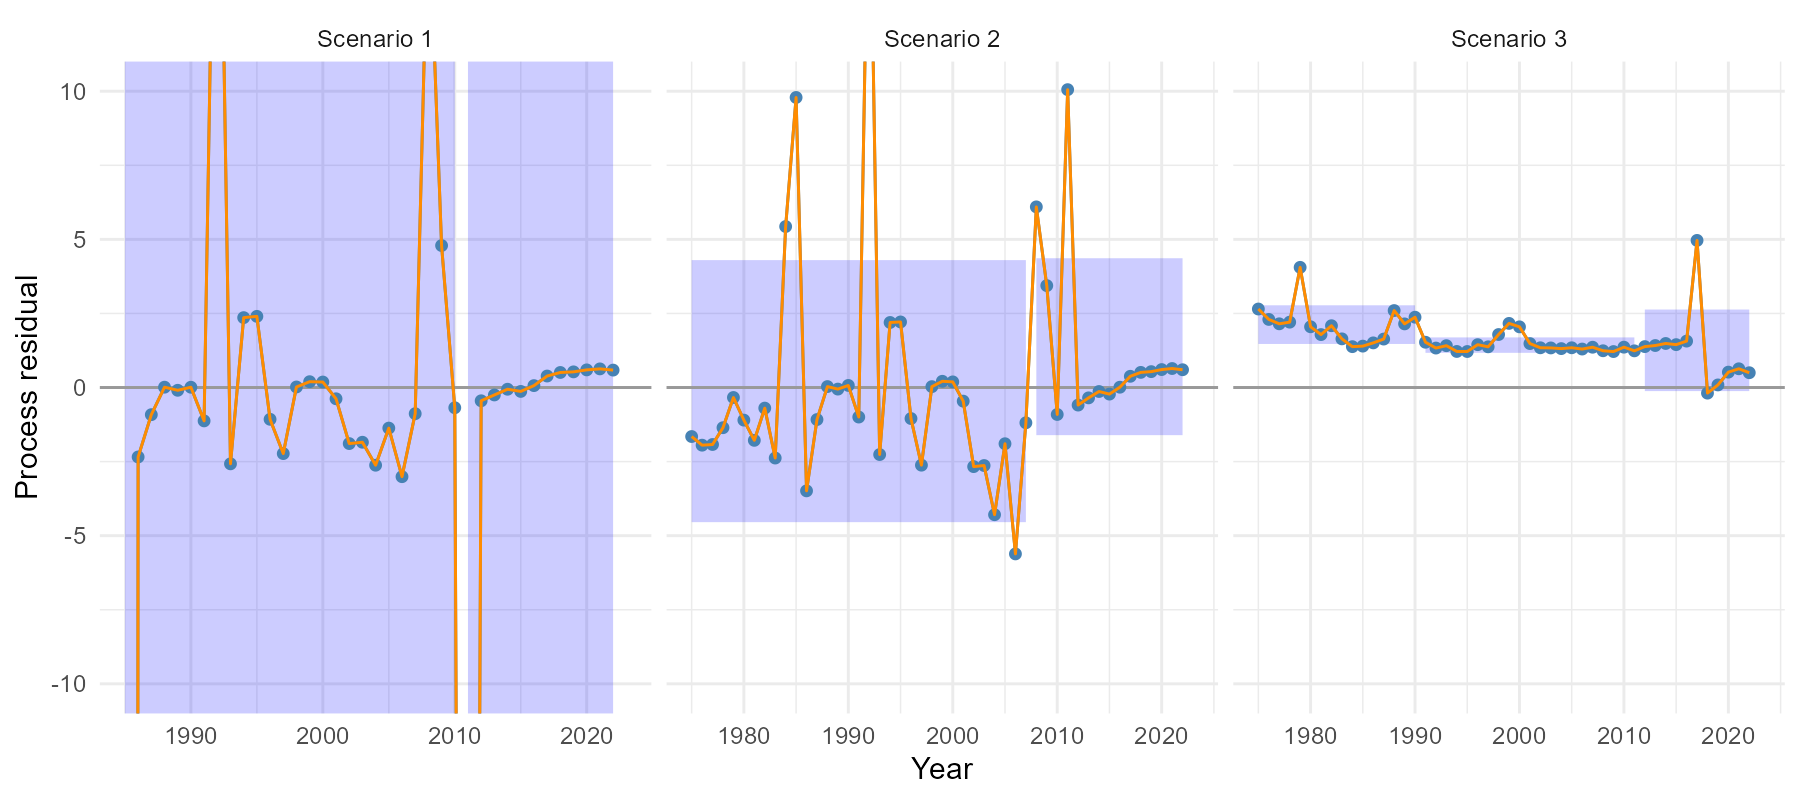
\includegraphics[width=0.92\linewidth]{figs/sma-fig-res-time-1.png}
  \caption{sma fig res time 1}
  \label{fig:robustness-sma-fig-res-time-1}
\end{figure}

\begin{figure}[H]
  \centering
  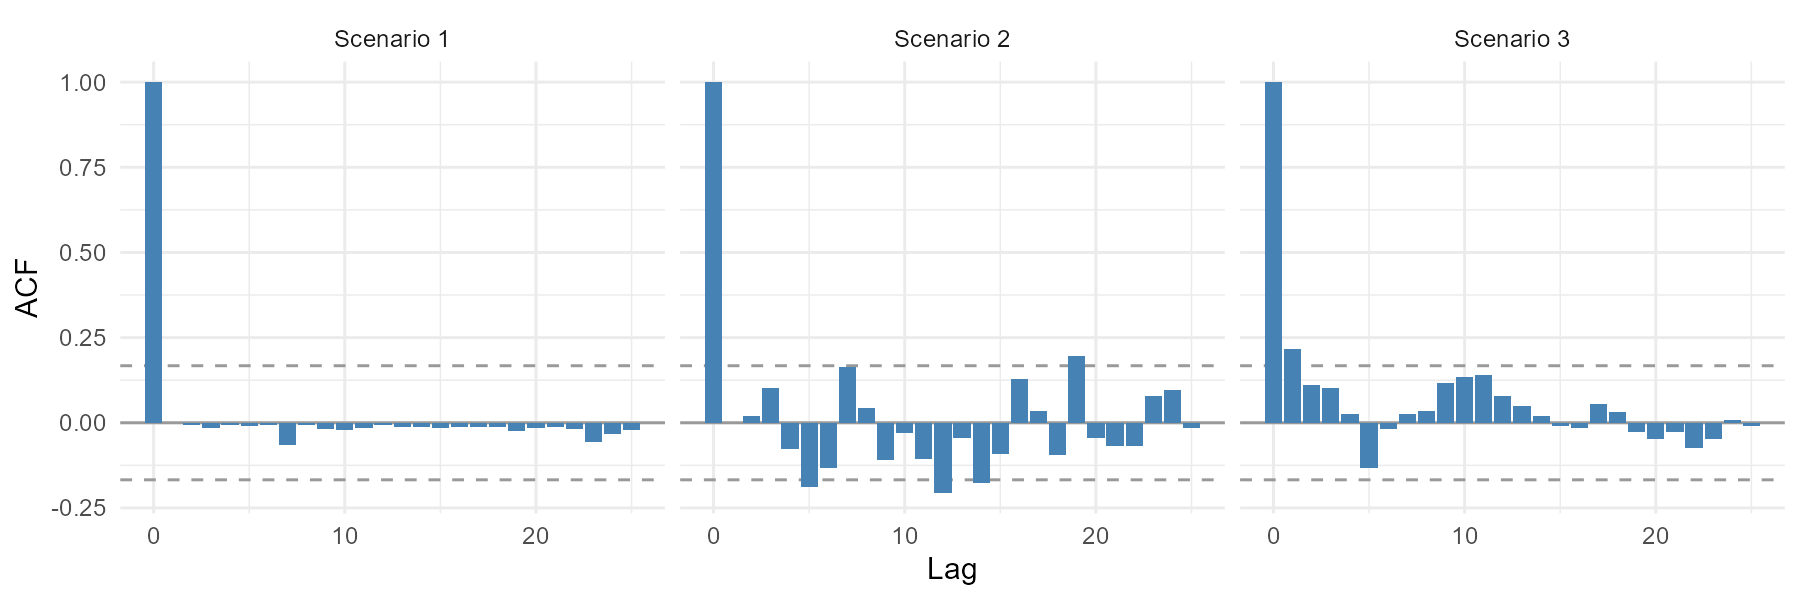
\includegraphics[width=0.92\linewidth]{figs/sma-fig-res-acf-1.png}
  \caption{sma fig res acf 1}
  \label{fig:robustness-sma-fig-res-acf-1}
\end{figure}

